% Chapter 1

\chapter{Introduction} % Main chapter title

\label{Chapter1} % For referencing the chapter elsewhere, use \ref{Chapter1} 

\lhead{Chapter 1. \emph{Introduction}} % This is for the header on each page - perhaps a shortened title

%----------------------------------------------------------------------------------------

\section{Introduction to Human Robot Interaction}
	Human-Robot Interaction (HRI) is a multidisciplinary field concerned with the “analysis, design, modeling, implementation and evaluation of robots for human use”\cite{fong2003collaboration}. \textbf{\emph{HRI is a challenging research field at the intersection of psychology, cognitive science, social sciences, artificial intelligence, computer science, robotics, engineering and human-computer interaction}}\cite{dautenhahn2007methodology}. The origin of HRI as a discrete problem was stated by 20$^{\text{th}}$ century author Isaac Asimov\cite{IssacAsimov} as he stated the \emph{Three Laws of Robotics} which every HRI designer should adhere to. While this acts as one of the first works proposing the guidelines for HRI, Goodrich \cite{goodrich2007human} instead in his extensive survey proposed two main types of HRI.
\begin{itemize}
\item Remote interaction/ Tele-operation: The human and the robot are not colocated and are separated spatially or even temporally (for example, the Mars Rovers are separated from earth both in space and time). 
\item Proximate interaction: The humans and the robots are co-located (for example, service robots may be in the same room as humans).
\end{itemize}
	Proximate interaction has gained importance due to the successful encounters of putting robots to work with human beings. It has led to the development of a new class of robots called Social Robots. The extensive survey conducted by Fong et al.,\cite{fong2003survey} on social robots araised some of the most important questions that have to be addressed in developing an engaging HRI system. Fong et al. \cite{fong2003survey} define that social robots are able to recognize each other and engage in social interactions; Breazeal et al.\cite{Breazeal:2002:DSR:515422} explain that a social robot is a robot which is able to communicate with humans in a personal way; Bartneck and Forlizzi \cite{bartneck2004design} describe that a social robot is an autonomous or semi-autonomous robot that interacts with humans by following some social behaviors; Hegel et al. \cite{hegel2009understanding} define that a social robot is a combination of a robot and a social interface. Summarizing all these Yan et al. \cite{yan2014survey} defines \emph{“A social robot is a robot which can execute designated tasks and the necessary condition turning a robot into a social robot is the ability to interact with humans by adhering to certain social cues and rules.”}. 
	
	The social robots already entered the human spaces as entertainers, educators\cite{NaoTheRobot} and caring agents\cite{ASKNao}. Given that social robotics has emerged as a promising field, designing and developing interaction systems need to be approached in a systematic manner wherein the robots should be able to understand and interact with the environment (man and materials) in a better way. To make it possible it is necessary to develop robotic systems with essential cognitive skills for efficient and natural interaction. Most often the onboard sensors on the robots fail to satisfy this demanding requirement. Hence consideration of using exteroceptive sensors to this purpose is important.  
	
	The HRI designers are from diverse backgrounds. So the tools needed to design behaviors of a social robot should be intuitive and user friendly. However when it comes to designing complex behaviors, traditional flow chart based approaches\cite{Choregraphe} increase the cognitive load of the users as they have to hand tailor all the data flow and reactiveness. More efficient tools are needed which could tackle this issue. 
	
	The main contribution of this thesis will be to develop an application independent experimental platform wherein a social robot will be equipped with essential perceptual ability to understand human motions. The behavior design of such a social robot will be made possible by efficient behavioral framework. The experimental platform will be used to design and evaluate the interaction between the social robot and the human.	

\section{Problem statements}
\label{sec:problem_statement}
	Human Robot interaction in social context has been studied rigorously due to the potential applications foreseen. For an effective interaction, the robot has to understand precisely its environment especially the human actions and deeds. The main focus of this study will be to understand the non-verbal aspect of the interaction (i.e., visual but not auditory). For visual understanding of human intention/motion the robot has to be equipped with exceptional perception system. Due to the various considerations like portability, on board processing capability and power consumption, most often the choice of on-board sensors is compromised. Eventually the precision of the sensor information from the onboard sensors are not enough for complete understanding of human motions. In such cases there is a need to use exteroceptive sensors which are practical to be used in a social scenario while at the same time powerful enough to satisfy the requirements. This problem boils down to \emph{Selection of Sensors} which are cheap, powerful and have sufficient tools for development. Moreover it requires the study on \emph{Human motion understanding} and \emph{Localization/Tracking} of humanoid robot.
	
	Secondly, the software frameworks available to design an interaction scenario are most often not scalable. This is mainly due to the trade-off between usability and capability of defining complex dynamic behaviors. There is a need to choose one among various available software frameworks, which allow us to define dynamic behaviors. This requires the study of existing \emph{Behavioral frameworks}.

	Thirdly, we have to put the perception system work under the framework of our choice and design appropriately the information flow. Finally there is also the need to evaluate the interaction by carefully designing the scenario and study the interaction metrics using data collection methods and statistical analysis. This requires the study of \emph{HRI design and evaluation techniques}.

	Considering all the above factors we could understand the need of an application independent experimental platform for studying the human-robot interaction understanding the human motions. Figure~\ref{fig:problemstatement} depicts the possible questions this thesis will try to investigate and propose solution. 

\begin{figure}[H]
\centering
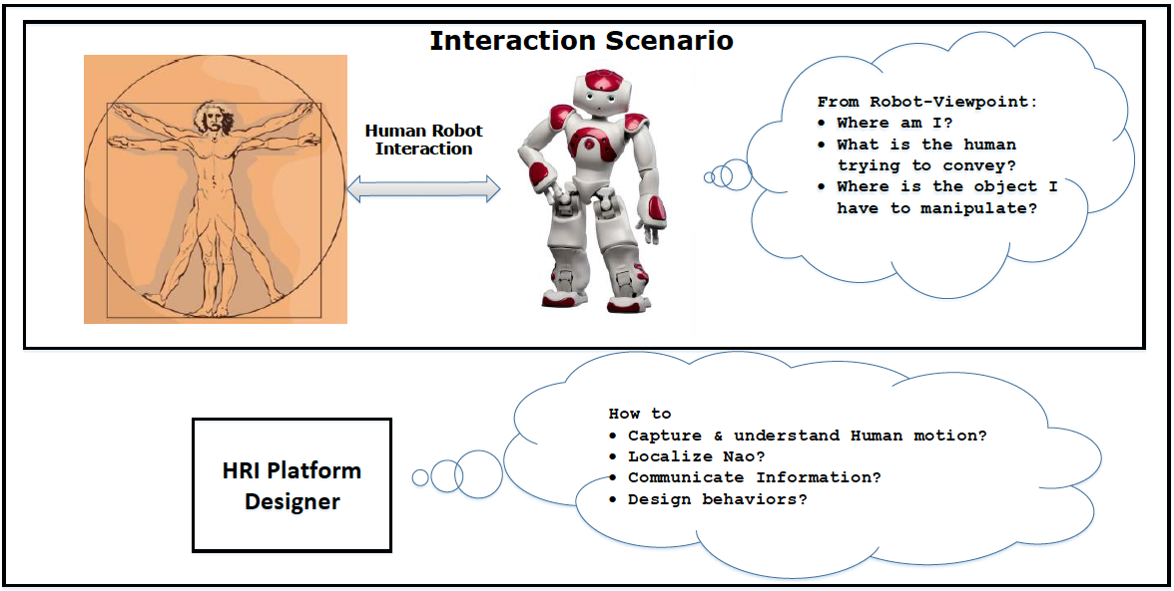
\includegraphics[width=\textwidth]{assets/ProblemStatement.png}
\caption{Concise depiction of problem statement}
\label{fig:problemstatement}
\end{figure}% 

\section{System requirements}
% \begin{figure}[H]
% \centering
% 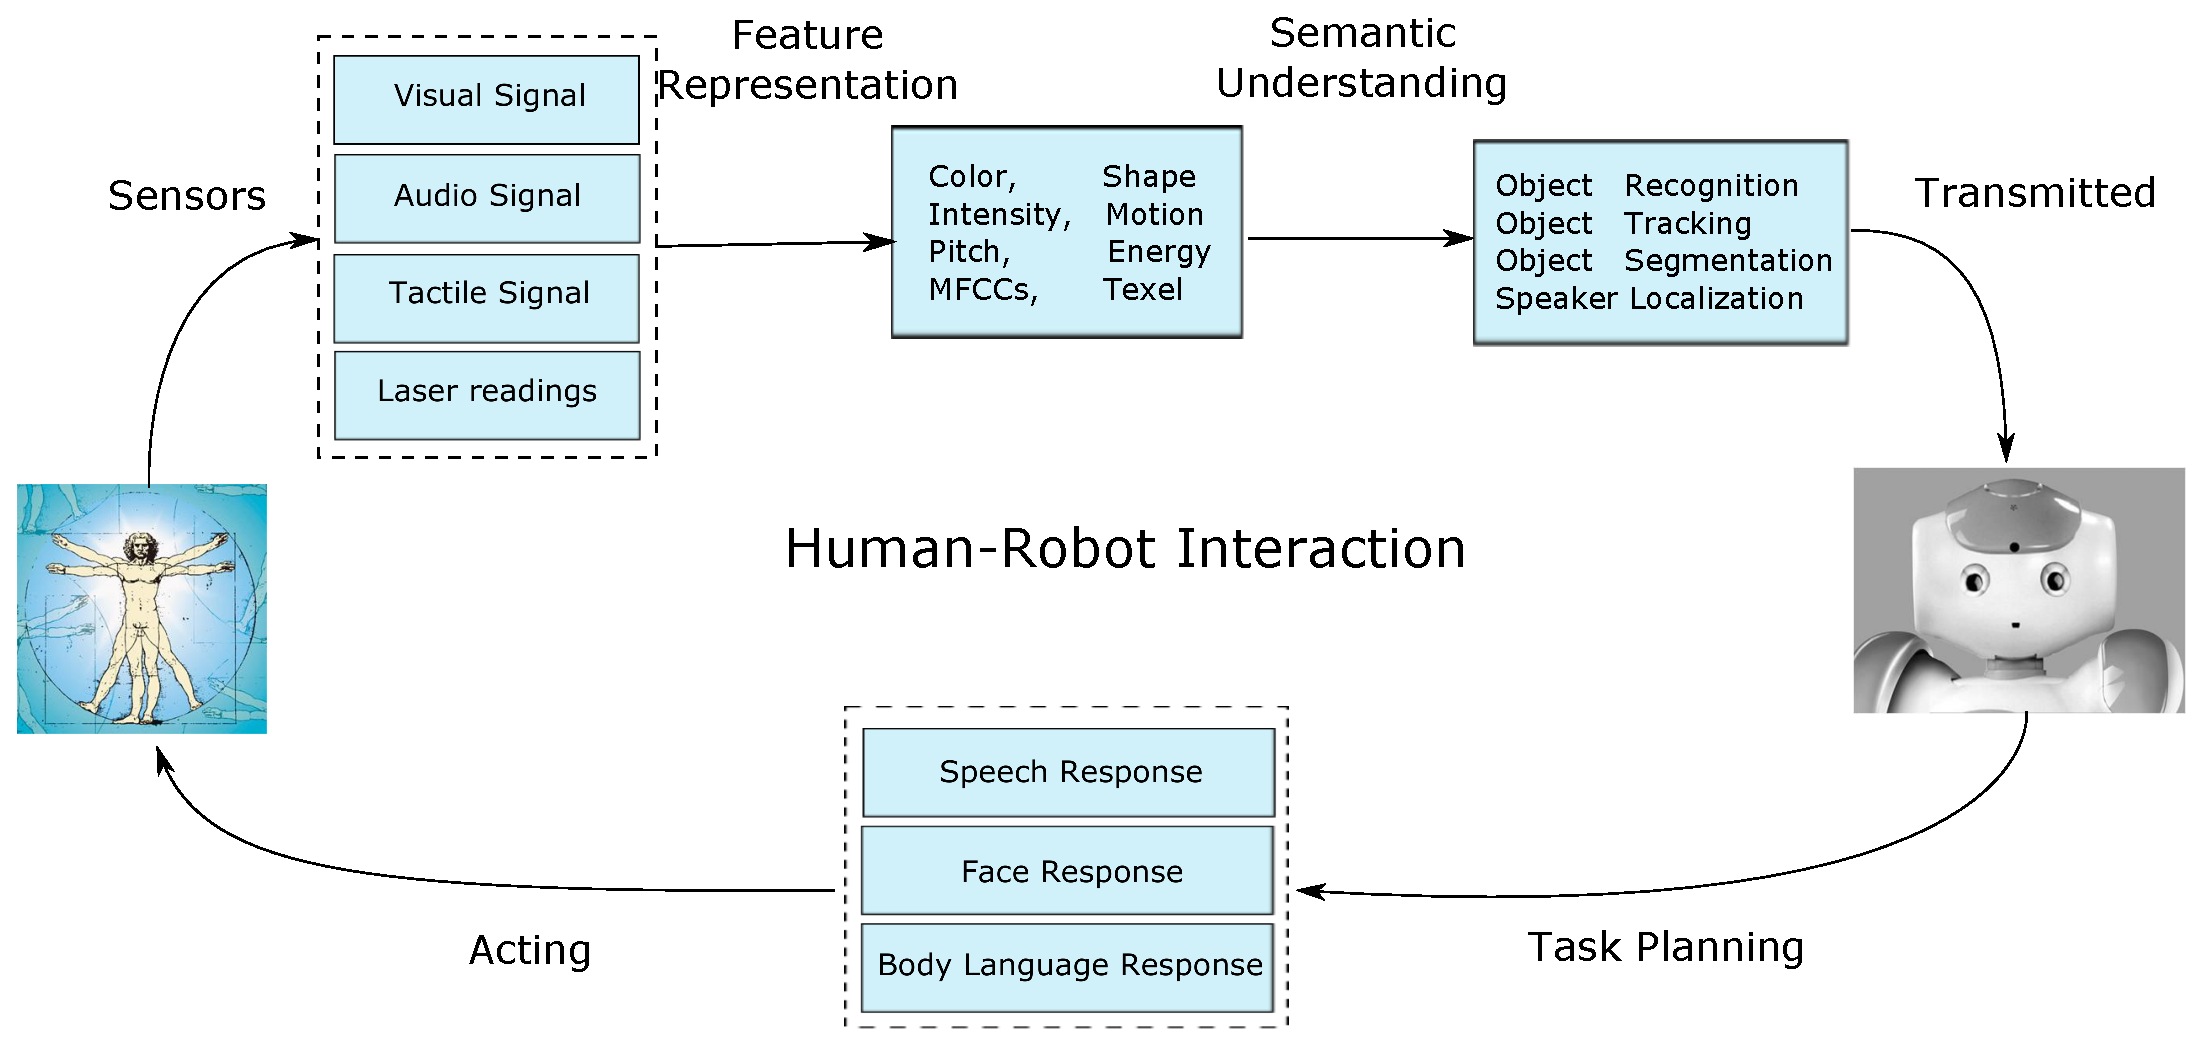
\includegraphics[width=1\textwidth]{assets/hri_perception.eps}
% \caption[Perception in Human Robot interaction]{Perception in Human Robot interaction. {Adopted from \cite{yan2014survey}}}
% \label{fig:hri_perception}
% \end{figure}
For human-robot interaction, perception is one of the most important capabilities. There have been recent surveys on perception methods for human-robot Interaction in the context of social robots \cite{yan2014survey}. There are four major classes of signals captured by a social robot. They are visual, audio, tactile and range sensors based signals. Depending on the task requirements, robots are equipped with one or many of these sensors and the sensors could be proprioceptive or exteroceptive. 
Our choice of perception system should satisfy the following requirements
\begin{itemize}
\item Precise 6-D localization of the robot and human(s) in the environment; For the 6D pose estimation we could use standalone or a combination of the following onboard sensors: Cameras, IMUs and Odometry sensors. However onboard sensors are erroneous.
\item Sensor data should facilitate the possibility of understanding human behaviors especially gestures and speech. For understanding complex human behaviors, the available on-board sensors and computing power are not enough. So we have to consider some exteroceptive sensors that satisfy this requirement. 
\item Practical for a social interaction scenario, cheap, and reliable.
\end{itemize}

\subsection{Perception system}
We are basically interested in capturing the human motion and speech. Microphones do not impose much contraints as it is ubiquitous these days and hence speech could be easuly captured. As far as human motions are concerned, Optical motion capture is one of the traditional ways of capturing them (System like VICON$^{\regmark}$ has been deployed to aquire the \emph{MOCAP} data). The system itself is huge, expensive to setup, need to equip the subject with reflective markers, suffers due to skin artifacts and has to be calibrated before using. Other devices which are commonly used to capture the kinematic information are \emph{Accelerometers} and \emph{Inertial Measurement Unit(IMU)}. The complete understanding of the human motion requires lot of such sensors to be attached on the human body which will make the human motions more constrained. 

Monocular cameras and laser rangefinders could be used for understanding human motions however each of them has advantages and disadvantages. The RGB-D cameras combining the strengths of optical cameras and laser range finders enable a complete perception solution. RGB-D cameras\cite{ren2013change} are active sensors that provide high resolution dense color and depth information at real time frame rates.
\begin{figure}[H]
\centering
%\begin{subfigure}[b]{0.5\textwidth}
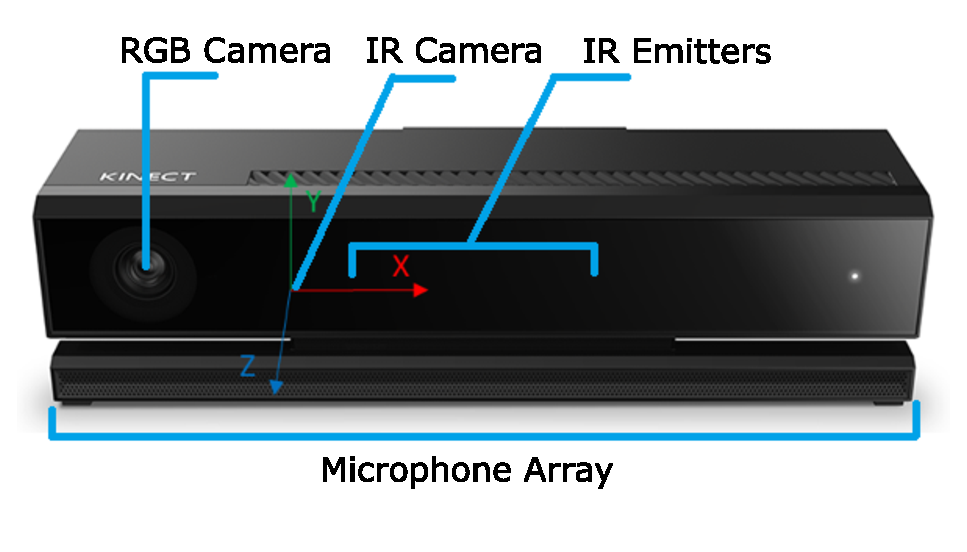
\includegraphics[width=0.5\textwidth]{assets/kinectv2_parts.eps}
%\caption{Kinect for Windows V2}
\label{fig:kinectv2}
%\end{subfigure}%
\caption[Kinect for Windows V2]{Kinect for Windows V2. {Adopted from manufacturer's site}}
%\label{fig:rgbd_sensors}
\end{figure}

A list of depth sensors available in the market along with their technical specification is shown in Table~\ref{table:rgbd_sensors} in Appendix~\ref{AppendixA}. Among them the Microsoft Kinect V2 \cite{Kinect2014} sensor has promising specifications and price. The Kinect comes with a powerful SDK \cite{KinectSDK2014} capable of performing skeleton tracking of upto 6 people (25 joints each) simultaneously out of the box. It also comes with the face detection, expression detection, gesture recognition and hand tracking. Additionally it has a microphone array which could be used for speech recognition using the Microsoft Speech SDK. It is also possible to build complex gestures using the Visual gesture builder and train the sensor to detect when it sees them later. 

\subsection{Humanoid robot}
Apart from a good perception system, we also need a very good humanoid robotics platform for evaluating the effectiveness of the system. It will be an added advantage if the chosen robotics platform is capable of exhibiting social behaviors and has already been accepted by a huge community of researchers and end-users. In recent times, the Nao humanoid robot \cite{NaoTheRobot} has been showing tremendous potential for its use in HRI studies. The robot NAO was developed in the year 2006 by Albebaran Robotics, the company which has proved itself in the development of interactive social robots.
\begin{figure}[H]
\centering
\begin{subfigure}[b]{0.25\textwidth}
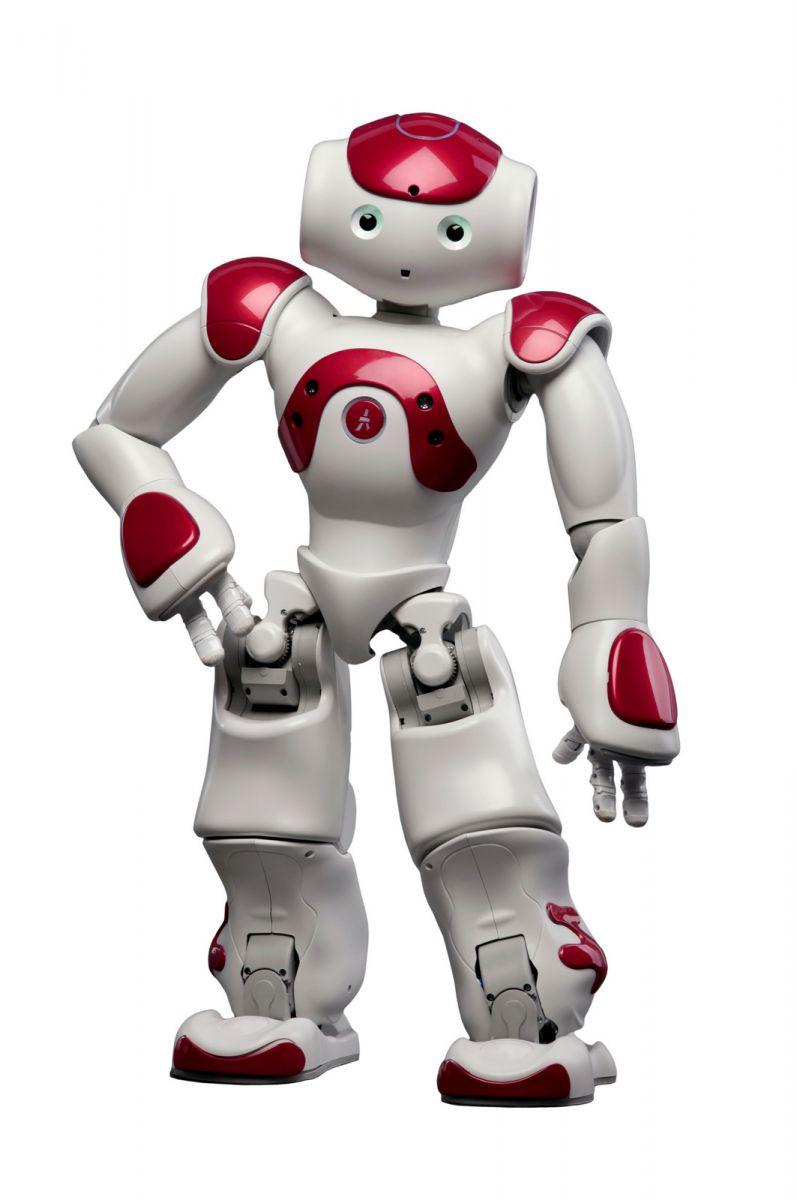
\includegraphics[width=\textwidth]{assets/nao_image1.jpg}
\caption{Robot appearance}
\label{fig:naojoint}
\end{subfigure}
\begin{subfigure}[b]{0.25\textwidth}
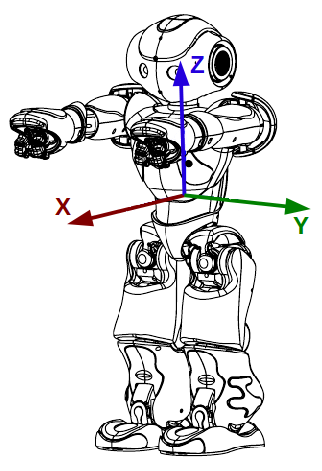
\includegraphics[width=\textwidth]{assets/hardware_inertialunit1.png}
\caption{Torso reference frame}
\label{fig:naoreference}
\end{subfigure}
\caption[NAO Humanoid Robot]{NAO Humanoid Robot. {Adopted from \cite{NaoTheRobot}}}
\label{fig:naorobot}
\end{figure}%
The intended scenarios include reception, assistance, home care, entertainment and even autism therapy. The technical specifications of the robot is shown in Fig~\ref{table:nao_spec}
\begin{table}[H]
\centering
\small
\caption{NAO humanoid platform technical specifications}
\label{table:nao_spec}
    \begin{tabular}{ | l | p{12cm} |}
    \hline
    \textbf{Category} & \textbf{Specification} \\
   \hline
  Version & NAO V50 H25 \\
                                          \hline
  Hardware & \begin{itemize}[leftmargin=*,topsep={0pt},itemsep={0pt},partopsep={0pt},parsep={0pt}] \item Body: 58 cm tall, 25 DOF composed of electric motors and actuators
  							\item Sensors: two cameras, four directional microphones, sonar rangefinder, two IR emitters and receivers, one inertial board, nine tactile sensors and eight pressure sensors
  							\item Communication devices: Voice synthesizer, LED lights, and 2 high-fidelity speakers
  							\item CPU: Intel ATOM 1.6ghz CPU 
  							\item Connectivity ; Ethernet and Wi-Fi
  							\item Power: 48.6-watt-hour battery that provides NAO with 1.5 or more hours of autonomy, depending on usage \end{itemize} \\
                                          \hline
                                          
  Motion  & \begin{itemize}[leftmargin=*,topsep={0pt},itemsep={0pt},partopsep={0pt},parsep={0pt}] \item Cartesian and Joint control. \item Omnidirectional walking, Whole body motion and Fall Manager \end{itemize} \\
                                          \hline
  
  Vision & \begin{itemize}[leftmargin=*,topsep={0pt},itemsep={0pt},partopsep={0pt},parsep={0pt}] \item Track, learn \& recognize images and faces. \item OpenCV support \end{itemize} \\
                                          \hline

  Audio & \begin{itemize}[leftmargin=*,topsep={0pt},itemsep={0pt},partopsep={0pt},parsep={0pt}] \item Sound Source Localization, Speech/Speaker recognition. \item Supports 19 languages.\end{itemize} \\
                                          \hline
  Software & \begin{itemize}[leftmargin=*,topsep={0pt},itemsep={0pt},partopsep={0pt},parsep={0pt}] \item OS: Linux kernel and supports NAOqi middleware
  							\item Tools: Choregraphe \cite{pot2009choregraphe} for designing behaviors
  							\item SDKs: C++/Python SDK for application developers \end{itemize} \\
                                          \hline
    \end{tabular}
\end{table}

\section{Main contributions}
\label{sec:contributions}

The main contribution of this thesis is a complete solution namely Indriya which offers end-to-end solution for designing human-robot interaction based on human behaviors. The overall system could be broken down into several sub-contributions most of which themselves are self-contained and independent. They are

\begin{itemize}
\item A distributed and modular \textbf{Application framework} which gives opportunity to interface multimodal sensor systems and diverse class of robots.
\item A simple and easy to understand \textbf{Behavior program model} in order to design reactive human robot interaction scenarios.
\item A \textbf{Behavior execution engine} which offers a powerful mechanism to execute the behavior program abstracting the trigger sources and responding hardwares.
\item An intuitive and easy to use \textbf{User interface} to design, execute and monitor interaction from broad range of client devices.
\end{itemize}

\section{Organization of the report}
\label{sec:organization}
The report is organized as follows. This chapter (Chapter~\ref{Chapter1}) introduced the topic of human-robot interaction and the problem statements of this thesis. Chapter~\ref{Chapter2} will give an overview of the tools and state of the art techniques related to the thesis. Chapter~\ref{Chapter3} will describe the software design principles used to develop the application infrastructure for the Indriya platform. The implementation details of the individual components of the platform exploiting the application infrastructure is described in Chapter~\ref{Chapter5}. Chapter~\ref{Chapter6} describes the evaluation of the system capabilties from a platform developer point of view. Chapter~\ref{Chapter7} discussed the protocol and results of the user study experiments. Finally Chapter~\ref{Chapter7} summarizes the project information, scope for prospective work and concluding remarks.